\chapter{DCE in a Periodic Potential} \label{ch:system}


\section{Circuit analysis for a 1D periodic potential quantum network}\label{sec:circ_an}
%


\subsection{Lagrangian}

\noindent
We now proceed to the study of the DCE in our proposed system, which consists of a periodic array of CPWs connected by SQUIDs (see Fig. \ref{fig:circuit_diagram}). To define the Lagrangian we discretize the system into 
segments $i$ of length $\Delta x$ with capacitance $\Delta x \, C_0$, inductance $\Delta x \, L_0$, and dynamical fluxes $\Phi_i(t)$ (see Ch.\ref{sec:SC_and_SQUIDs}).
Assuming symmetric SQUIDs, the Lagrangian for this system is (cp. Johansson \cite{Johansson2010_DCE}, Eq.\,(5))
\color{red}\{note edits: use index $n$ for SQUIDs instead of $s$\} \color{black}
%
\begin{figure}[h]\label{fig:circuit_diagram}
    %Hand-drawn placeholder figures. Made to work out placement, size, and captions while high resolution figures are generated.
    \centering
    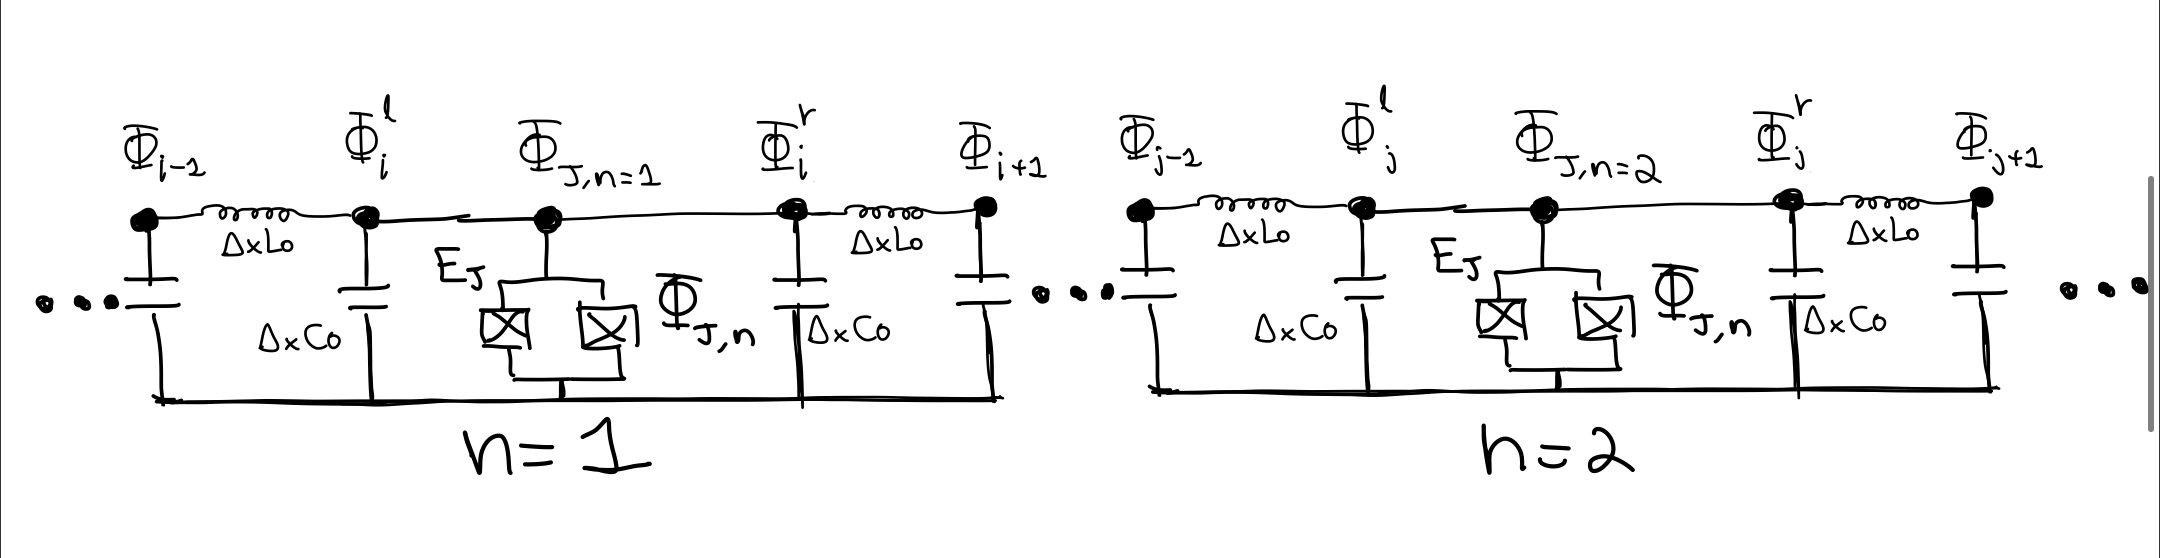
\includegraphics[width=\textwidth, keepaspectratio]{figures/circuit_diagram.png}
    \caption{Circuit diagram for a periodic lattice consisting of CPWs connected by symmetric SQUIDs at lattice sites $n$. 
    The dynamical fluxes $\Phi_i$ and $\Phi_{J,\,n}$ characterize the system.}
\end{figure}
%
\begin{equation} \label{eq:lagn1}
\begin{split}
\mathcal{L} = \, & \frac{1}{2} \sum_i \left( \Delta x \, C_{0} \left(\dot{\Phi}_{i}\right)^{2} \, - \, 
\frac{\left(\Phi_{i+1}-\Phi_{i}\right)^{2}}{\Delta x \, L_{0}} \right)  \\[2mm]
& + \sum_n \left[ \frac{1}{2} \, C_{J,\,n} \left(\dot{\Phi}_{J,\,n} \right)^{2} \, + \, 
E_{J,\,n}(t) \cos\left(2\pi \frac{\Phi_{J,\,n}}{\Phi_0} \right) \right]
\end{split}
\end{equation}
%
where a dot over a symbol indicates a time derivative, e.g., 
$\displaystyle \dot{\Phi}_i = \frac{\partial}{\partial t} \Phi_i$.
The terms on the r.h.s.\,of the first line of Eq.\,(\ref{eq:lagn1}) describe sections of the CPW between the SQUIDs. 
The second line of Eq.\,(\ref{eq:lagn1}) describes a periodic array of SQUIDs indexed by $n$ 
with effective capacitance $C_{J,\,n}$ and flux $\Phi_{J,\,n}$ at node $n$, where 
the subscript $J$ stands for the two Josephson junctions of a SQUID.
$\Phi_0 = h / (2 e)$ is the magnetic flux quantum.
The SQUIDs are separated by 
distance $\ell$ corresponding to the lattice constant of the one-dimensional (1D) SQUID array. 
The Josephson energy $E_{J,\,n}(t)$ of SQUID $n$ is tunable
by the externally applied magnetic flux $\Phi_{\text{ext},\,n}(t)$ through the SQUID 
(cp. Johansson, Eq.\,(6)): 
%
\begin{equation} \label{eq:squidenergy}
    E_{J,\,n}(t) = 2 \, \epsilon_{J,\,n} 
    \left\vert \cos\left(\pi \, \frac{\Phi_{\text{ext},\,n}(t)}{\Phi_0}\right)\right\vert \, \, ,
\end{equation}
%
where $\epsilon_{J,\,n}$ is a constant energy parameter.

We assume that the plasma frequency $\omega_p$ of the SQUIDs far exceeds other characteristic frequencies 
in the circuit so that oscillations in the phase across the SQUIDs have small amplitude, i.e., 
$\Phi_{J,\,n} / \Phi_0 \ll 1$,
and the SQUIDs are operated in the phase regime where $E_{J,\,n} \gg (2e)^2 / (2C_{J,\,n})$. 
Using $\Phi_{J,\,n} / \Phi_0 \ll 1$ one may expand the cosine in Eq.\,(\ref{eq:lagn1}), 
resulting in a Lagrangian quadratic in $\Phi_{J,\,n}$ (dropping terms $E_{J,\,n}(t)$ 
independent of $\Phi_{J,\,n}$)
%
\begin{equation} \label{eq:lagn2}
\begin{split}
\mathcal{L} = \, & \frac{1}{2} \sum_i \left( \Delta x \, C_{0} \left(\dot{\Phi}_{i}\right)^{2} \, - \, 
\frac{\left(\Phi_{i+1}-\Phi_{i}\right)^{2}}{\Delta x \, L_{0}} \right)  \\[2mm]
& + \frac{1}{2} \sum_n \left( C_{J,\,n} \left(\dot{\Phi}_{J,\,n} \right)^{2} \, - \, 
 \left(\frac{2 \pi}{\Phi_0} \right)^2 E_{J,\,n}(t) \, \left( \Phi_{J,\,n} \right)^2 
\right) \, \, .
\end{split}
\end{equation}
%
Note that we make the identification $\Phi_i^{\,l} = \Phi_{J,\,n} = \Phi_i^{\,r}$ for the flux at SQUID $n$, 
where $\Phi_i^{\,l}$ and $\Phi_i^{\,r}$ are the fluxes at adjacent nodes to the left ($l$) and right ($r$) of 
node $n$, respectively (see Fig. \ref{fig:circuit_diagram}). 

From now on, we assume that the intrinsic device parameters of all SQUIDs are equal, i.e., 
$C_{J,\,n} = C_J$, $\epsilon_{J,\,n} = \epsilon_J$ for all $n$ in Eqs.\,(\ref{eq:lagn2}), (\ref{eq:squidenergy}).  
Moreover, we assume that the SQUID energy $E_{J,\,n}(t)$ in Eq.\,(\ref{eq:squidenergy}) 
can be expanded in a static part plus harmonic drive 
(cp. Johansson, text page 6 bottom left)
\color{red}
\{Note: harmonic drive doesn't need to be weak since we don't do perturbation theory as in Johansson\}
\color{black}
%
\begin{equation} \label{eq:energyexp1}
E_{J,\,n}(t) = E_J^0 + \delta E_{J,\,n} \cos(\Omega \, t + \varphi_n) 
\end{equation}
%
where $\delta E_{J,\,n} < E_J^0$ and $\Omega$ is the frequency of the external drive 
$\Phi_{\text{ext}}(t)$ in Eq.\,(\ref{eq:squidenergy}).
As indicated in Eq.\,(\ref{eq:energyexp1}), we assume that the {\em static} part 
$E_J^0$ of $E_{J,\,n}(t)$ is the same for all SQUIDs (i.e., indepedent of $n$). 
This assumption is crucial for our 
treatment of the {\em static} system (realized by a static applied magnetic flux $\Phi_{\text{ext}}$
for all SQUIDs) as a 1D periodic lattice with period $\ell$. However, the 
time-dependent contribution in Eq.\,(\ref{eq:energyexp1})
may be modulated along the SQUID array, i.e., may differ for different SQUIDs $n$,
in terms of amplitudes $\delta E_{J,\,n}$ and phases $\varphi_n$.
This allows us to externally control the DCE radiation generated in the SQUID array
by varying the parameters $\delta E_{J,\,n}$ and $\varphi_n$.
However, we will assume for simplicity that the drive frequency 
is the same for all SQUIDs, i.e., $\Omega_n = \Omega$ for all $n$.
That is, we consider an amplitude modulation but no frequency modulation of the 
time-dependent contribution in Eq.\,(\ref{eq:energyexp1}). 
%
%
%\begin{equation} \label{eq:energyexp2}
%E_{J,\,n}(t) \equiv E_J(t) = E_J^0 + \delta E_J \cos(\Omega \, t) \qquad \text{for all} \, \, \, \, n \, \, . 
%\end{equation}
%
%With these assumptions, the Lagrangian (\ref{eq:lagn2}) takes the form
%
%\begin{equation} \label{eq:lagn3}
%\begin{split}
%\mathcal{L} = \, & \frac{1}{2} \sum_i \left( \Delta x \, C_{0} \left(\dot{\Phi}_{i}\right)^{2} \, - \, 
%\frac{\left(\Phi_{i+1} - \Phi_{i}\right)^{2}}{\Delta x \, L_{0}} \right)  \\[2mm]
%& + \frac{1}{2} \sum_n \left( C_J \left(\dot{\Phi}_{J,\,n} \right)^{2} \, - \, 
% \left(\frac{2 \pi}{\Phi_0} \right)^2 E_{J,\,n}(t) \, \left( \Phi_{J,\,n} \right)^2 
%\right) \, \, .
%\end{split}
%\end{equation}
%
%with $E_{J,\,n}(t)$ from Eq.(\ref{eq:energyexp1}). 

\subsection{Quantization of the dynamic flux in the periodic SQUID array}

To quantize the system, we first transform the Lagrangian $\mathcal{L}$ in Eq.\,(\ref{eq:lagn2})
into a Hamiltonian $\mathcal{H}$ by a Legendre transformation.
To this end, it is convenient to temporarily consider the fluxes $\Phi_i^{\,l}$, $\Phi_i^{\,r}$, and $\Phi_{J,\,n}$ 
at SQUIDs $n$ as independent dynamic variables (cp.\,remark below Eq.(\ref{eq:lagn2})) and define 
%
\begin{equation} \label{eq:ham1}
\mathcal{H} = \sum_{i} \frac{\partial\mathcal{L}}{\partial\dot{\Phi}_i} \, \dot{\Phi}_i 
\, + \, \sum_{n} \frac{\partial\mathcal{L}}{\partial\dot{\Phi}_{J,\,n}} \, \dot{\Phi}_{J,\,n}
\, - \, \mathcal{L} \, \, , 
\end{equation}
%
resulting in
%
\begin{equation} \label{eq:ham2}
\begin{split}
\mathcal{H} = \, & \frac{1}{2} \sum_i \left( \frac{P_i^{\,2}}{\Delta x \, C_{0}} \, + \, 
\frac{\left(\Phi_{i+1} - \Phi_{i}\right)^{2}}{\Delta x \, L_{0}} \right)  \\[2mm]
& + \frac{1}{2} \sum_n \left( \frac{\left(P_{J,\,n}\right)^2}{C_{J}} \, + \, 
 \left(\frac{2 \pi}{\Phi_0} \right)^2 E_{J,\,n}(t) \, \left( \Phi_{J,\,n} \right)^2 
\right)
\end{split}
\end{equation}
%
with the canonical conjugate momenta
%
\begin{subequations} \label{eq:mom}
\begin{eqnarray} 
P_i = \frac{\partial\mathcal{L}}{\partial\dot{\Phi}_i} = \Delta x \, C_0 \, \dot{\Phi}_i \label{eq:moma} \, \, \, , \\[2mm]
P_{J,\,n} = \frac{\partial\mathcal{L}}{\partial\dot{\Phi}_{J,\,n}} =  C_J \, \dot{\Phi}_{J,\,n} \, \, \,  . \label{eq:momb}
\end{eqnarray}
\end{subequations}
%
At this point, we identify again 
$\Phi_i^{\,l} = \Phi_{J,\,n} = \Phi_i^{\,r}$ and $P_i^{\,l} = P_{J,\,n} = P_i^{\,r}$
for the fluxes and conjugate momenta at SQUIDs $n$.
The system is quantized by turning the fluxes $\Phi_i(t)$ and conjugate momenta $P_i(t)$ 
to operators $\hat{\Phi}_i(t)$, $\hat{P}_i(t)$ with equal-time commutation relations
%
\begin{equation} \label{eq:cr} 
\left[\hat{\Phi}_i(t), \hat{P}_j(t) \right] = i \hbar \delta_{ij} \, \, , \quad 
\left[\hat{\Phi}_i(t), \hat{\Phi}_j(t) \right] = 0 \, \, , \quad 
\left[\hat{P}_i(t), \hat{P}_j(t) \right] = 0 \, \, \, , 
\end{equation}
%
with the identifications mentioned above; for example, 
$\left[\hat{\Phi}_i^{\,l}, \hat{P}_{J,\,n} \right] = 
\left[\hat{\Phi}_i^{\,r}, \hat{P}_{J,\,n} \right] = i \hbar$ (see Fig. \ref{fig:circuit_diagram}).

%%%%%%%%%%%%%%%%%%%%%%%%%%%%%%%%%%%%%%%%%%%%%%%%%%%%%%

\subsection{Wave equation and boundary conditions}

In the CPW between the SQUIDs, the Heisenberg equation of motion 
$\displaystyle \frac{d}{dt} \hat{P}_i = \frac{i}{\hbar} \left[\hat{\mathcal{H}}, \hat{P}_i \right]$ 
results in, using Eqs.\,(\ref{eq:ham2}) - (\ref{eq:cr}), 
%
\begin{equation} \label{eq:eom1}
C_0 L_0 \, \frac{d^2}{dt^2} \hat{\Phi}_i \, = \, 
\frac{1}{(\Delta x)^2} \left(\hat{\Phi}_{i+1} - 2 \hat{\Phi}_i +  \hat{\Phi}_{i-1} \right) \, \, .
\end{equation}
%
In the continuum limit $\Delta x \to 0$ writing $\hat{\Phi}_i(t) \to \hat{\Phi}(x,t)$ 
with a continuous position variable $x$ the r.h.s.\,of Eq.\,(\ref{eq:eom1}) becomes
$\displaystyle \frac{\partial^2\hat{\Phi}(x,t)}{\partial x^2}$. 
We thus obtain the wave equation for the dynamic flux operator
$\hat{\Phi}(x,t)$ in the CPW between the SQUIDs,
%
\begin{equation} \label{eq:eom2}
\frac{\partial^2\hat{\Phi}(x,t)}{\partial t^2} - v^2 \, \frac{\partial^2\hat{\Phi}(x,t)}{\partial x^2} = 0 \, \, ,
\end{equation}
%
where $v = 1 / \sqrt{C_0 L_0}$ is the wave propagation speed in the CPW.
We note that, in the continuum limit $\Delta x \to 0$, 
the momentum operator conjugate to $\hat{\Phi}(x,t)$ is given by,
instead of Eq.\,(\ref{eq:moma}), 
%
\begin{equation} \label{eq:mom2} 
\hat{\overline{P}}(x,t) := \frac{\hat{P}_{i}(t)}{\Delta x} = 
C_0 \, \frac{\partial}{\partial t} \hat{\Phi}(x,t)
\end{equation}
%
with equal-time commutation relations
%
\begin{equation} \label{eq:cr2} 
\left[\hat{\Phi}(x,t), \hat{\overline{P}}(x',t) \right] = i \hbar \delta(x - x') \, \, , \quad 
\left[\hat{\Phi}(x,t), \hat{\Phi}(x',t) \right] = 0 \, \, , \quad 
\left[\hat{\overline{P}}(x,t), \hat{\overline{P}}(x',t) \right] = 0 \, \, \, , 
\end{equation}
%
where $\delta(x)$ is the 1D delta function (with units of $1/x$).

Similarly, at the $n$th SQUID site, the Heisenberg equations of motion
$\displaystyle \frac{d}{dt} \hat{P}_{J,\,n} = \frac{i}{\hbar} \left[\hat{\mathcal{H}}, \hat{P}_{J,\,n} \right]$ 
results in, using Eqs.\,(\ref{eq:ham2}) - (\ref{eq:cr}) with the identifications noted below
Eq.\,(\ref{eq:momb}), 
\color{red} \{note edits: BC doesn't contain $\hbar$ (was wrong in early write-up, later corrected) and 
terms $\hat{\Phi}_{i+1}$, $\hat{\Phi}_{i-1}$ have the same sign (was right in write-up)\}
\color{black}
%
\begin{equation}\label{eq:BC_discrete}
C_{J} \, \frac{d^2}{dt^2} \hat{\Phi}_{J,\,n} \, + \left(\frac{2 \pi}{\Phi_{0}} \right)^{2} E_{J,\,n}(t) \, \hat{\Phi}_{J, \, n}
\, + \frac{1}{L_{0}} 
\left( \frac{\hat{\Phi}_{J,\,n} - \hat{\Phi}_{i-1}}{\Delta x} - \frac{\hat{\Phi}_{i+1} - \hat{\Phi}_{J,\,n}}{\Delta x} \right)
\, = \, 0 \, \, ,
\end{equation}
%
where $\hat{\Phi}_{i-1}$ and $\hat{\Phi}_{i+1}$ are adjacent nodes to the left and right of 
$\hat{\Phi}_i^{\,l} = \hat{\Phi}_{J,\,n} = \hat{\Phi}_i^{\,r}$, respectively
\color{red}
(Figure X). 
\color{black}
In the continuum limit $\Delta x \to 0$ we obtain the boundary condition for $\hat{\Phi}(x, t)$ 
at the SQUID sites $x_n$
%
\begin{equation}\label{eq:BC_field_orig}
C_{J} \, \frac{\partial^2 \hat{\Phi}(x_n, t)}{\partial t^2} \, + 
\left(\frac{2 \pi}{\Phi_{0}}\right)^{2} E_{J,\,n}(t) \, \hat{\Phi}(x_n, t) \, + 
\frac{1}{L_{0}}\left(\left.\frac{\partial \hat{\Phi}(x, t)}{\partial x}\right|_{x_n^{-}}
- \, \left.\frac{\partial \hat{\Phi}(x,t)}{\partial x}\right|_{x_n^{+}}\right) \, = \, 0 \, \, ,
\end{equation}
%
where $\displaystyle \left.\frac{\partial \hat{\Phi}}{\partial x}\right|_{x_n^{-}}$
denotes a derivative from the left ($-$) of $x_n$ evaluated at $x_n$ and
$\displaystyle \left.\frac{\partial \hat{\Phi}}{\partial x}\right|_{x_n^{+}}$
denotes a derivative from the right ($+$) of $x_n$ evaluated at $x_n$
\color{red}
(Figure Y). 
\color{black}
The SQUID energy $E_{J,\,n}(t)$ is given by Eq.\,(\ref{eq:energyexp1}). 

In the absence of the SQUIDs, i.e., $C_J = E_{J,\,n}(t) = 0$, 
Eq.\,(\ref{eq:BC_field_orig}) shows that $\partial \hat{\Phi} / \partial x$ is 
continuous everywhere, and the solution of the wave equation (\ref{eq:eom2})
are simple harmonic waves $\hat{\Phi}(x,t) \sim \exp\left[i (q x - \omega \, t) \right]$
with angular frequency $\omega$, 1D wave vector $q$, and dispersion relation 
$\omega(q) = v |q|$
\footnote{We denote the 1D wave vector for the free CPW by the symbol $q$ to distinguish it 
from the wave vector $k$ of the Bloch waves obtained for the periodic SQUID array in the static case
obtained in Section \ref{subsec:kpsol}.}.
However, in the presence of the SQUIDs the boundary condition  
(\ref{eq:BC_field_orig}) introduces discontinuities (jumps) of $\partial \hat{\Phi} / \partial x$ 
at the SQUID sites $x_n = \ell n$ and $\hat{\Phi}(x,t)$ are no longer simple harmonic waves
(cp.\,Section \ref{sec:kp} below) 

%%%%%%%%%%%%%%%%%%%%%%%%%%%%%%%%%%%%%%%%%%%%%%%%%%%%%%%%%%%%%%%%%%%%%%%%%%%%%%%%%%%%%%%%%%%%%%%%%%%%%%
%%%%%%%%%%%%%%%%%%%%%%%%%%%%%%%%%%%%%%%%%%%%%%%%%%%%%%%%%%%%%%%%%%%%%%%%%%%%%%%%%%%%%%%%%%%%%%%%%%%%%%

\section{Relation to the Kronig-Penney model in the static case} 
\label{sec:kp}

\subsection{Boundary condition in frequency domain}

In this section we consider the static case, in which $\delta E_{J,\,n} = 0$ in Eq.\,(\ref{eq:energyexp1})
and the SQUID energy $E_{J,\,n} = E_J^0$ is constant. In this case, the boundary condition 
(\ref{eq:BC_field_orig}) is given by
%
\begin{equation}\label{eq:BC_field_static_orig}
C_{J} \, \frac{\partial^2 \hat{\Phi}(x_n, t)}{\partial t^2} \, + 
\left(\frac{2 \pi}{\Phi_{0}}\right)^{2} E_J^0 \, \hat{\Phi}(x_n, t) \, + 
\frac{1}{L_{0}}\left(\left.\frac{\partial \hat{\Phi}(x, t)}{\partial x}\right|_{x_n^{-}}
- \, \left.\frac{\partial \hat{\Phi}(x,t)}{\partial x}\right|_{x_n^{+}}\right) \, = \, 0 \, \, . \quad \text{(static)}
\end{equation}
%
We will generally work in the frequency domain instead of the time domain by 
expanding $\hat{\Phi}(x, t)$ in harmonic modes 
$\hat{\Phi}_{\omega}(x, t) = \hat{\varphi}(x,\omega) \exp(i \omega \, t)$ of frequency $\omega$
(see Eq.\,(\ref{eq:flux_field_orig}) below).
In the frequency domain the boundary condition for the static case in Eq.\,(\ref{eq:BC_field_static_orig}) 
translates to a boundary condition for $\hat{\varphi}(x,\omega)$:
%
\begin{equation}\label{eq:BC_freq_static}
- C_{J} \, \omega^2 \hat{\varphi}(x_n, \omega) \, + 
\left(\frac{2 \pi}{\Phi_{0}}\right)^{2} E_J^0 \, \hat{\varphi}(x_n, \omega) \, + 
\frac{1}{L_{0}}\left(\left.\frac{\partial \hat{\varphi}(x, \omega)}{\partial x}\right|_{x_n^{-}}
- \, \left.\frac{\partial \hat{\varphi}(x,\omega)}{\partial x}\right|_{x_n^{+}}\right) \, = \, 0 \, \, .
\quad \text{(static)}
\end{equation}
%
Note that Eq.\,(\ref{eq:BC_freq_static}) only holds in the static case because 
for time-dependent SQUID energy $E_{J,\,n}(t)$ the term $E_{J,\,n}(t) \, \hat{\Phi}(x_n, t)$ 
in Eq.\,(\ref{eq:BC_field_orig}) generates a coupling of modes with different frequencies $\omega$.

%The physical unit of the field operator $\hat{\Phi}(x,t)$ in Eq.\,(\ref{eq:BC_field_orig}) is determined 
%by the first commutation relation in Eq.\,(\ref{eq:cr2}) with $\hat{\overline{P}}(x,t)$ from Eq.\,(\ref{eq:mom2}).
%This implies that the physical unit of the field operator is determined by  
%%
%\begin{equation} \label{eq:phiunit} 
%\left[ \hat{\Phi}^2 \right] = \left[ \frac{\hbar \cdot \text{s}}{C_0 \cdot \text{m}} \right] \, \, .
%\end{equation} 
%%
In large parts of this thesis we will use unitless variables by expressing lenghts in units of $\ell$
and times in units of $\ell/v$ where $\ell$ is the distance between SQUIDs in the periodic array 
\color{red}
(Figure X)
\color{black}
and $v = 1 / \sqrt{C_0 L_0}$ is the speed of light in the CPW in Eq.\,(\ref{eq:eom2}).  
%
%We thus can introduce a unitless field operator by
%%
%\begin{equation} \label{eq:ufo2}
%\hat{\phi}(x,t) := \sqrt{\frac{2 C_0 v}{\hbar}} \, \hat{\Phi}(x,t) \, \, ,
%\end{equation}
%
%where here $x$, $t$ are the unitless versions of position and time and 
%the factor of 2 in the square root is for convenience.
The boundary condition (\ref{eq:BC_freq_static}) can be expressed in terms of unitless parameters
by multiplying both sides of Eq.\,(\ref{eq:BC_freq_static}) by $L_0 \, \ell$, resulting in
\footnote{We use the same symbol $x$ for the original position variable and its 
unitless version (position in units of $\ell$) to keep the notation reasonably simple.}
%
\begin{equation}\label{eq:BC_freq_static_unitless}
\epsilon(\omega) \hat{\varphi}(n, \omega) \, = \, 
\left.\frac{\partial \hat{\varphi}(x, \omega)}{\partial x}\right|_{n^{+}}
- \, \left.\frac{\partial \hat{\varphi}(x,\omega)}{\partial x}\right|_{n^{-}}
\quad \text{(static, unitless)}
\end{equation}
%
where $n$ is the position of the $n$th SQUID in units of $\ell$ and 
%
\begin{equation} \label{eq:epsilon}
\epsilon(\omega) \, = \, L_0 \, \ell \left[ - C_{J} \, \omega^2 + 
\left(\frac{2 \pi}{\Phi_{0}}\right)^{2} E_J^0 \right] 
\end{equation}
%
is a unitless parameter.

From now on we assume for simplicity that the SQUID plasma frequency $\omega_p$ is sufficiently 
large so that we can neglect the term $C_{J} \, \omega^2$ in Eq.\,(\ref{eq:epsilon}) compared to 
the other term \cite{Johansson2010_DCE}
(cp.\,text below Eq.\,(\ref{eq:squidenergy})), i.e., we will use the $\omega$-independent parameter
%
\begin{equation} \label{eq:epsilon2}
\epsilon \, = \, L_0 \, \ell \left(\frac{2 \pi}{\Phi_{0}}\right)^{2} E_J^0 \, \, .
\end{equation}

\color{red}
\{Give typical value for $\epsilon$ for different choices of $\ell$\}
\color{black}

%%%%%%%%%%%%%%%%%%%%%%%%%%%%%%%%%%%%%%%%%%%%%%%%%%%%%%%%%%%%%%

\subsection{Relation to the Kronig-Penney model}
\label{subsec:kp}

The Kronig-Penney model is a simplified model for an electron in a 1D 
periodic potential
\color{red}
(cite: quantum mechanics textbook).
\color{black}
Modeling the periodic potential as a Dirac comb with amplitude $u>0$
and lattice constant $\ell$, the time-independent Schr\"odinger equation reads
%
\begin{equation} \label{eq:kpschrod}
- \frac{\hbar^2}{2 m} \frac{d^2}{dx^2} \psi(x) + u \, \ell \sum_n \delta(x - n \ell) \psi(x) = E \psi(x) \, \, , 
\end{equation}
%
where $\psi(x)$ is the wave function, $m$ the mass, and $E$ the energy 
of the electron.
This equation can be made unitless by multiplying both sides
with $\displaystyle \frac{2 m \, \ell^2}{\hbar^2}$ which yields
%
\begin{equation} \label{eq:kpschrod_unitless}
- \psi''(x) + \epsilon \sum_n \delta(x - n) \psi(x) = {\cal E} \psi(x) \, \, , \quad \text{(Kronig-Penney, unitless)} 
\end{equation}
%
where the position $x$ is expressed in units of $\ell$, the prime symbol denotes a derivative
with respect to $x$, and
%
\begin{equation} \label{eq:kpschrod_param}
\epsilon = \frac{2 m u \, \ell^2}{\hbar^2} \, \, , \quad {\cal E} = \frac{2 m E \ell^2}{\hbar^2}
\end{equation}
%
are unitless (re-scaled) versions of $u$ and $E$.
Integrating Eq.\,(\ref{eq:kpschrod_unitless}) over a small region about  
$n$ according to $\displaystyle \int_{n - \delta x}^{n + \delta x} dx$ \,
followed by the limit $\delta x \to 0$ yields
a boundary condition at $n$ in terms of a jump of the first derivative $\psi'(x)$
\color{red}
(cite: quantum mechanics textbook)
\color{black}
%
\begin{equation}\label{eq:kpjump}
\epsilon \psi(n,{\cal E}) \, = \, 
\left. \psi'(n,{\cal E}) \right|_{n^{+}} - \left. \psi'(n,{\cal E}) \right|_{n^{-}} \, \, .
\quad \text{(Kronig-Penney, unitless)}
\end{equation}
%
Comparison with Eq.\,(\ref{eq:BC_freq_static_unitless}) shows that the form of the boundary
conditions for the field operator $\hat{\varphi}(x, \omega)$ in the 1D periodic SQUID array
(static case)
and the electron wave function $\psi(x,{\cal E})$ in the Kronig-Penney model 
are identical. However,
in the absence of the periodic potential in the Kronig-Penney model, i.e., $u=\epsilon=0$, 
the solution of Eq.\,(\ref{eq:kpschrod_unitless}) 
are harmonic waves $\psi(x,{\cal E}) \sim \exp(i q x)$ with 1D wave vector $q$ and dispersion relation 
${\cal E}(q) = q^2$ (corresponding to 
$\displaystyle E(q) = \hbar^2 q^2 / (2 m)$ in original variables).
In contrast, for the free CPW we found the dispersion relation
$\omega(q) = |q|$ in unitless variables (corresponding to $\omega(q) = v |q|$ in original variables,
see text in paragraph below Eq.\,(\ref{eq:BC_field_orig}))
%
\footnote{We denote the 1D wave vector for the free CPW by the symbol $q$ to distinguish it 
from the wave vector $k$ of the Bloch waves obtained for the periodic SQUID array in the static case
obtained in Section \ref{subsec:kpsol}.}.
%
That is, $\omega(q)$ in the free CPW is a linear 
function of $q$ instead of quadratic, which is a consequence of the fact that the particles 
in the CPW are massless photons whereas the electrons in the Schr\"odinger equation (\ref{eq:kpschrod})
have a finite mass $m$. 

However, except for this difference of the dispersion relation, the solution for the 
field operator $\hat{\varphi}(x, \omega)$ in the 1D periodic SQUID array 
with boundary condition (\ref{eq:BC_freq_static_unitless}) at the SQUID sites $n$ for the static case
is analogous to that of the Kronig-Penney model. 

%%%%%%%%%%%%%%%%%%%%%%%%%%%%%%%%%%%%%%%%%%%%%%%%%%%%%%%%%%%%%

\subsection{Solution of the Kronig-Penney-type model for the 1D SQUID array in the static case}
\label{subsec:kpsol}

\color{red}
\{This subsection is more drafty, needs to be finalized\}
\color{black}

\noindent
This subsection uses unitless variables
by expressing lenghts in units of $\ell$ and times in units of $\ell/v$ as discussed above
\footnote{We use the same symbols $x$, $q$, $k$, $\omega$, etc.\,for the original variables 
and their unitless versions to keep the notation reasonable simple. It will be clear from 
the context and/or by explicit marking which version of variables are used.}.

In the frequency domain, the equation of motion for the CPW between the SQUIDs is given by
Eq.\,(\ref{eq:eom2}) with 
$\Phi_{\omega}(x, t) = \varphi(x,\omega) \exp(i \omega \, t)$ 
(see text below Eq.\,(\ref{eq:BC_field_static_orig})), which results in
\footnote{In this subsection we skip the hat symbol for operators since the operator property 
of $\varphi(x,\omega)$ is not used.}
%
\begin{equation} \label{eq:eom3}
\varphi''(x,\omega) + \omega^2 \varphi(x,\omega) = 0 \, \, .
\end{equation}
% 
The boundary conditions at the SQUID sites $n$, in the static case, 
are given by Eq.\,(\ref{eq:BC_freq_static_unitless}):
%
\begin{equation}\label{eq:BC_freq_static_unitless_2}
\epsilon \varphi(n, \omega) \, = \, 
\left.\frac{\partial \varphi(x, \omega)}{\partial x}\right|_{n^{+}}
- \, \left.\frac{\partial \varphi(x,\omega)}{\partial x}\right|_{n^{-}} \quad \text{for all integer} \, \, \, n \, \, \, .
\end{equation}
%
Note that, by using unitless variables, the only system-specific parameter in 
Eqs.\,(\ref{eq:eom3}), (\ref{eq:BC_freq_static_unitless_2}) is the unitless energy parameter 
$\epsilon$ in Eq.\,(\ref{eq:epsilon2}). 

The solution of the Kronig-Penney-type model defined by 
Eqs.\,(\ref{eq:eom3}), (\ref{eq:BC_freq_static_unitless_2}) is presented in detail in  
\color{red}
a Mathematica notebook enclosed as Appendix M.
\color{black}
The strategy is to use an ansatz for $\varphi_n(x)$ for each section $n$ of the CPW
between SQUIDs as a linear combination of right-moving
and left-moving plane waves with 1D wave vector $q>0$ as in a free CPW:
\color{red}
\{See "KP model Geshkenbein", page 5 ("our version")\}
\color{black}
%
\begin{equation} \label{eq:kpansatz}
\varphi_n(x) \, = \, A_n \, \exp\left[i q (x-n) \right] \, + \, 
B_n \, \exp\left[-i q (x-n) \right] \, \, , \quad n-1 < x < n \, \, ,
\end{equation}
%
and to determine the $n$-dependent coefficients $A_n$, $B_n$ by the boundary conditions 
(\ref{eq:BC_freq_static_unitless_2}) using a transfer matrix approach 
\color{red}
(cite: Geshkenbein).
\color{black}
(The extra terms $\exp(- i q n)$, $\exp(i q n)$ in Eq.\,(\ref{eq:kpansatz}) were introduced 
for computational convenience, see 
\color{red}
Mathematica notebook in Appendix M).
\color{black}

\color{red} 
{\bf Move everything related to the static Kronig-Penney model here. 
Briefly discuss the Bloch functions and dispersion relation $\omega(k)$ in unitless variables. 
I tentatively moved some text to this subsection, needs to be edited (can do this later)}.  
\color{black}

We find solutions of the Kronig-Penney-type model defined by 
Eqs.\,(\ref{eq:eom3}), (\ref{eq:BC_freq_static_unitless_2})
in terms of Bloch functions
%
\begin{equation} \label{eq:psi1}
\psi_k(x) = e^{i k x} u_k(x) \, \, ,   
\end{equation}
%
where $k$ is a 1D Bloch wave vector, which depends in a nontrivial way on the wave vector 
$q$ used in the ansatz (\ref{eq:kpansatz}). Since
$\omega = q$ in unitless variables (corresponding to $\omega(q) = v q$ in original variables,
and using $q>0$ in Eq.\,(\ref{eq:kpansatz})),
the dependence $k(q)$ directly translates to a dependence $k(\omega)$, corresponding to the 
inverse of the dispersion relation $\omega(k)$ for the Kronig-Penney-type model.
The function $u_k(x)$ in Eq.\,(\ref{eq:psi1}) has period $1$, that is, $u_k(x + n) = u_k(x)$ 
for all integers $n$.
Thus, $u_k(x)$ is completely specified by the domain $x \in [0,1]$ and periodic extension
beyond this domain. 
The functions $k(\omega)$ and $u_k(x)$, $0 < x < 1$, are calculated in the 
\color{red}
Mathematica notebook in Appendix M
\color{black}
using a transfer matrix approach. 






The Bloch functions $\psi_k(x)$ in Eq.\,(\ref{eq:psi1}) are unitless, orthogonal with respect to 
the 1D wave vector $k$, and normalized such that
%
\begin{equation} \label{eq:psi1_norm_orig}
\int_{-\infty}^{\infty} dx \, \psi^*_k(x) \psi_{k'}(x) = 2 \pi \, \delta(k - k') \, \, .
\end{equation}
%
The introduction of a periodic potential leads to a Bloch band structure similar to the one for electrons in 
solid state physics (see section \ref{sec:KP_in_SS}) with energy bands determined by the dispersion relation
\begin{equation}\label{eq:disp_rel}
    \cos{k} = \cos{\omega} + \frac{\epsilon}{2\omega}\sin{\omega}
\end{equation}
%
with $\epsilon$ defined in Eq.\,(\ref{eq:epsilon}) 
\color{red}
\{need to check if $\lambda = \epsilon$\}
\color{black}


\begin{equation}\label{eq:lambda}
\lambda = \left(\frac{L_0}{\hbar}\right)  
\left[-\omega^2 C_{J}+\hbar\left(\frac{2 \pi}{\Phi_{0}}\right)^{2} E_{j}^0\right].
\end{equation}
%

Allowed energy states correspond to solutions of Eq. \ref{eq:disp_rel} with frequencies $\omega$ such that
%
\begin{equation}\label{eq:bands_condition}
    \left|\cos{\omega} + \frac{\lambda}{2\omega}\sin{\omega}\right|\leq 1.
\end{equation}

Mention/explain extended zone scheme.


%%%%%%%%%%%%%%%%%%%%%%%%%%%%%%%%%%%%%%%%%%%%%%%%%%%%%%%%%%%%%%%%%%%%%%%%%%%%%%%%%%%%%%%%%%%%%%%%%%%%%%%%%%%%%%
%%%%%%%%%%%%%%%%%%%%%%%%%%%%%%%%%%%%%%%%%%%%%%%%%%%%%%%%%%%%%%%%%%%%%%%%%%%%%%%%%%%%%%%%%%%%%%%%%%%%%%%%%%%%%%


\section{Dynamical Casimir radiation in the periodic SQUID array}\label{sec:dcr}
%
%Let us first consider the background periodic potential in the static case where we apply a 
%DC drive so that the SQUID energy $E_J(t) = E_J^0$ is constant. 

\color{blue}
\subsection{Dynamic flux field in second quantized form}

\noindent
We start this Section using original variables for clarity, and later turn to unitless variables to 
simplify the notation and facilitate the numerical implementation. 
For each section $n$ of the CPW between SQUIDs $n-1$ and $n$ we expand the field operator $\hat{\Phi}(x,t)$
introduced below Eq.\,(\ref{eq:eom1}), with boundary conditions (\ref{eq:BC_field_orig}) at the SQUID sites 
$x_n = n \ell$, in second quantized form using annihilation and creation operators $\hat{a}_n(k)$ and 
${\hat a}_n^\dagger(k)$:
%
\begin{equation} \label{eq:flux_field_orig}
    \hat{\Phi}_n(x,t) = \sqrt{\frac{\hbar}{2 C_0}} 
    \int_{-\infty}^{\infty}\frac{dk}{2 \pi} \frac{1}{\sqrt{\omega(k)}}
    \left\{ \hat{a}_n(k) \psi_k(x) \, e^{-i \omega(k) \, t} \, + \, 
    \hat{a}_n^{\dagger}(k) \psi_k^*(x) \, e^{i \omega(k) \, t} \right\} \, \, , \quad x_{n-1} < x < x_n \, \, ,
\end{equation}
%
where $\psi_k(x)$ are Bloch functions with dispersion relation $\omega(k)$ defined for the {\em static}
system as in Section \ref{sec:kp}, and we use the extended zone scheme to label the energy bands 
(see subsection \ref{subsec:kp}). The Bloch functions have the form (see Eq.\,(\ref{eq:psi1})) 
%
\begin{equation} \label{eq:psi2}
\psi_k(x) = e^{i k x} u_k(x) \, \, ,   
\end{equation}
%
where $u_k(x)$ has period $\ell$ so that $u_k(x + n \ell) = u_k(x)$
for all integers $n$.
The Bloch functions $\psi_k(x)$ are unitless and orthogonal with respect to 
the 1D wave vector $k$. They are normalized such that
%
\begin{equation} \label{eq:psi1_norm_orig2}
\int_{-\infty}^{\infty} dx \, \psi^*_k(x) \psi_{k'}(x) = 2 \pi \, \delta(k - k')
\end{equation}
%
and fulfill the completeness relation
%
\begin{equation} \label{eq:psi1_comp_orig}
\int_{-\infty}^{\infty}\frac{dk}{2 \pi} \, \psi_{k}(x) \psi^*_k(x') = \delta(x-x') \, \, .
\end{equation}

In Eq.\,(\ref{eq:flux_field_orig})
we introduce the index $n$ to indicate that $\hat{\Phi}_n(x,t)$ is defined in the domain
$x_{n-1} < x < x_n$ corresponding to section $n$ of the CPW. Field operators $\hat{\Phi}_n(x,t)$,
$\hat{\Phi}_{n+1}(x,t)$ in adjacent sections $n$, $n+1$ are coupled by the boundary condition 
(\ref{eq:BC_field_orig}) at the SQUID site $x_n$.
The operators $\hat{a}_n(k)$, $\hat{a}_n^{\dagger}(k)$ act as expansion coefficients of 
$\hat{\Phi}_n(x,t)$ in section $n$.
Conversely, the Bloch functions $\psi_k(x)$ are defined for the global system by construction 
and do not depend on $n$.

For each section $n$ of the CPW the annihilation and creation operators in 
Eq.\,(\ref{eq:flux_field_orig}) obey the commutation relations
%
\begin{equation} \label{eq:cra_orig}
    \left[ \hat{a}_n(k),{\hat a}_n^\dagger(k') \right] = 2 \pi \delta(k - k')
\end{equation}
%
and have units of $\text{length}^{1/2}$.
The prefactor $\displaystyle{\sqrt{\frac{\hbar}{2 C_0}}}$ in Eq.\,(\ref{eq:flux_field_orig}) 
is determined by the equal-time commutation relation for section $n$ of the CPW,
$\left[\hat{\Phi}_n(x,t), \hat{\overline{P}}_n(x',t) \right] = i \hbar \delta(x - x')$ 
in Eq.\,(\ref{eq:cr2}), using Eqs.\,(\ref{eq:cra_orig}) and (\ref{eq:psi1_comp_orig}).

Equation (\ref{eq:flux_field_orig}) incorporates our strategy to find the radiation created by the 
dynamical Casimir effect (DCE) in the 1D SQUID array with time-dependent drive, Eq.\,(\ref{eq:energyexp1}). 
...

\color{black}

We now rewrite Eq.\,(\ref{eq:flux_field_orig}) in terms of unitless variables 
by expressing lenghts in units of $\ell$ and times in units of $\ell/v$
as outlined in \color{red} Section X:  \color{black}  
%
\begin{equation} \label{eq:flux_field}
    \hat{\phi}_n(x,t) = 
    \int_{-\infty}^{\infty}\frac{dk}{2 \pi} \frac{1}{\sqrt{\omega_k}}
    \left[ \hat{a}_n(k) \psi_k(x)e^{-i \omega(k) \, t} + 
    \hat{a}_n^{\dagger}(k) \psi_k^*(x) e^{i \omega(k) \, t} \right]
\end{equation}
%
with the unitless field operator in compartment $n$ of the periodic array
%
\begin{equation} \label{eq:ufo}
\hat{\phi}_n(x,t) := \sqrt{\frac{2 C_0 v}{\hbar}} \, \hat{\Phi}_n(x,t) \, \, .
\end{equation}
%
Unitless annihilation and creation operators are defined by $\hat{a}_n(k)/\sqrt{\ell}$ 
and ${\hat a}_{n}^\dagger(k) / \sqrt{\ell}$ and again denoted by
$\hat{a}_n(k)$, ${\hat a}_{n}^\dagger(k)$ to keep the notation simple. 
They obey the commutation relations 
%
\begin{equation} \label{eq:cra}
    \left[ \hat{a}_n(k),{\hat a}_{n'}^\dagger(k') \right] = \delta_{nn'} \, 2 \pi \delta(k - k') \, \, .
\end{equation}
%
Note that all variables in Eq.\,(\ref{eq:flux_field}) become unitless by expressing lengths in units of $\ell$ and times in units of $\ell/v$. The following results are then valid for any general system exhibiting time-dependent harmonic modulations in a periodic lattice. The variables that are unique to our superconducting circuit setup are and the speed of propagation in the CPW $v$, the length of the CPW segments $\ell$, and the variable $\lambda$, which determines the strength of the potential encountered at our SQUID sites. It follows then that subsequent analysis applies to any other physical realization, with corresponding physical values of $\ell$, $v$, and $\lambda$.

\section{Static Solution}\label{eq:Static_Flux}
%
Given the time dependence of the flux field $\hat{\phi}_n(x,t)$, in Eq. (\ref{eq:flux_field}) we can write our boundary condition (\ref{eq:BC_field_orig}) as
%
\begin{equation}\label{eq:BC_field}
\left[-\omega^2 C_{J}+\hbar\left(\frac{2 \pi}{\Phi_{0}}\right)^{2} E_{j}^0\right]\hat{\phi}_n(x,t) -\frac{\hbar}{L_{0}}\left(\left.\frac{\partial \hat{\phi}_n(x,t)}{\partial x}\right|_{x_n^{+}}-\left.\frac{\partial \hat{\phi}_n(x,t)}{\partial x}\right|_{x_n^{-}}\right)=0.
\end{equation}
%
We proceed to obtain solutions for the problem with applied static magnetic flux. Taking the Fourier transform of the field \ref{eq:flux_field}, expanded in terms of the bloch waves
\begin{equation}\label{eq:field_FT}
    \hat{\phi}_n(x, \mu) = \int_{-\infty}^\infty \hat{\phi}_n(x,t) e^{i\mu t} dt
\end{equation}
%
We obtain the following forms for the field at the $n$th CPW segment:
\begin{subequations} \label{eq:phi_FT}
\begin{eqnarray}
    \hat{\phi}_n(x, \mu) =  \left|\left.\frac{d\omega}{dk}\right|_{\omega=\mu}\right|^{-1}\frac{1}{\sqrt{\mu}}\biggl\lbrace \hat{a}_n^R(K) \psi^R_K(x) + \hat{a}_n^L(K)\psi_K^L(x)\biggr\rbrace, &\text{for } \mu > 0, \label{eq:phi_FT_a}\\
    \hat{\phi}_n(x, \mu) = \left|\left.\frac{d\omega}{dk}\right|_{\omega=\mu}\right|^{-1}\frac{1}{\sqrt{|\mu|}}\biggl\lbrace [\hat{a}^R_n(K)]^\dagger \left[\psi^R_K(x)\right]^* + [\hat{a}_n^L(K)]^\dagger\left[\psi_K^L(x)\right]^*\biggr\rbrace, &\text{for } \mu < 0. \label{eq:phi_FT_b}
\end{eqnarray}
\end{subequations}
%
Where we use $k_{\mu} = k_{-\mu} = k_{|\mu|}$ defined $K = |k|$, and have used forms of the Bloch functions (see Appendix \ref{ch:appendix_bloch})
%
\begin{equation}\label{eq:bloch_waves}
    \psi_{K}^R (x) =e^{iKx} u_{K}^{(1)}(x), \hspace{12pt}  \psi_{K}^L(x) =e^{-iKx} u_{K}^{(2)}(x),
\end{equation}
%
as well as 
\begin{equation}
    \hat{a}_n(K) = 
    \begin{cases}
    \hat{a}_n^R(K), &\text{if k > 0,}\\
    \hat{a}_n^L(K), &\text{if k < 0.}
    \end{cases}
\end{equation}
%
Taking the Fourier transform of our $n$th site boundary condition (\ref{eq:BC_field}) for positive frequencies (\ref{eq:phi_FT_a}), we arrive at a relation,

\begin{equation}\label{eq:BC_static_1}
\begin{split}
    \left[-\mu^2 C_{J}+\hbar\left(\frac{2 \pi}{\Phi_{0}}\right)^{2} E_{j}^0\right].
    \left\lbrace\hat{a}^R(K) \psi^R_K(n) + \hat{a}^L(K) \psi^L_K(n) \right\rbrace =
    \\[2mm]
       \left(\frac{\hbar}{L_0}\right) 
    \left\lbrace\hat{b}^R(K) \left.\frac{\partial \psi^R_K(x)}{\partial x}\right|_{x=n^-} +\hat{b}^L(K) \left.\frac{\partial \psi^L_K(x)}{\partial x}\right|_{x=n^-}\right\rbrace.
    \\[2mm]
    -
    \left(\frac{\hbar}{L_0}\right) 
    \left\lbrace\hat{a}^R(K) \left.\frac{\partial \psi^R_K(x)}{\partial x}\right|_{x=n^+} +\hat{a}^L(K) \left.\frac{\partial \psi^L_K(x)}{\partial x}\right|_{x=n^+} \right\rbrace
\end{split}
\end{equation}
%
Where we have omitted the $n$ subscript in our annihilation/creation operators and defined $\hat{b} = \hat{a}_{n+1}$.
%
\begin{figure}\label{fig:boundary_schematic}
    \centering
    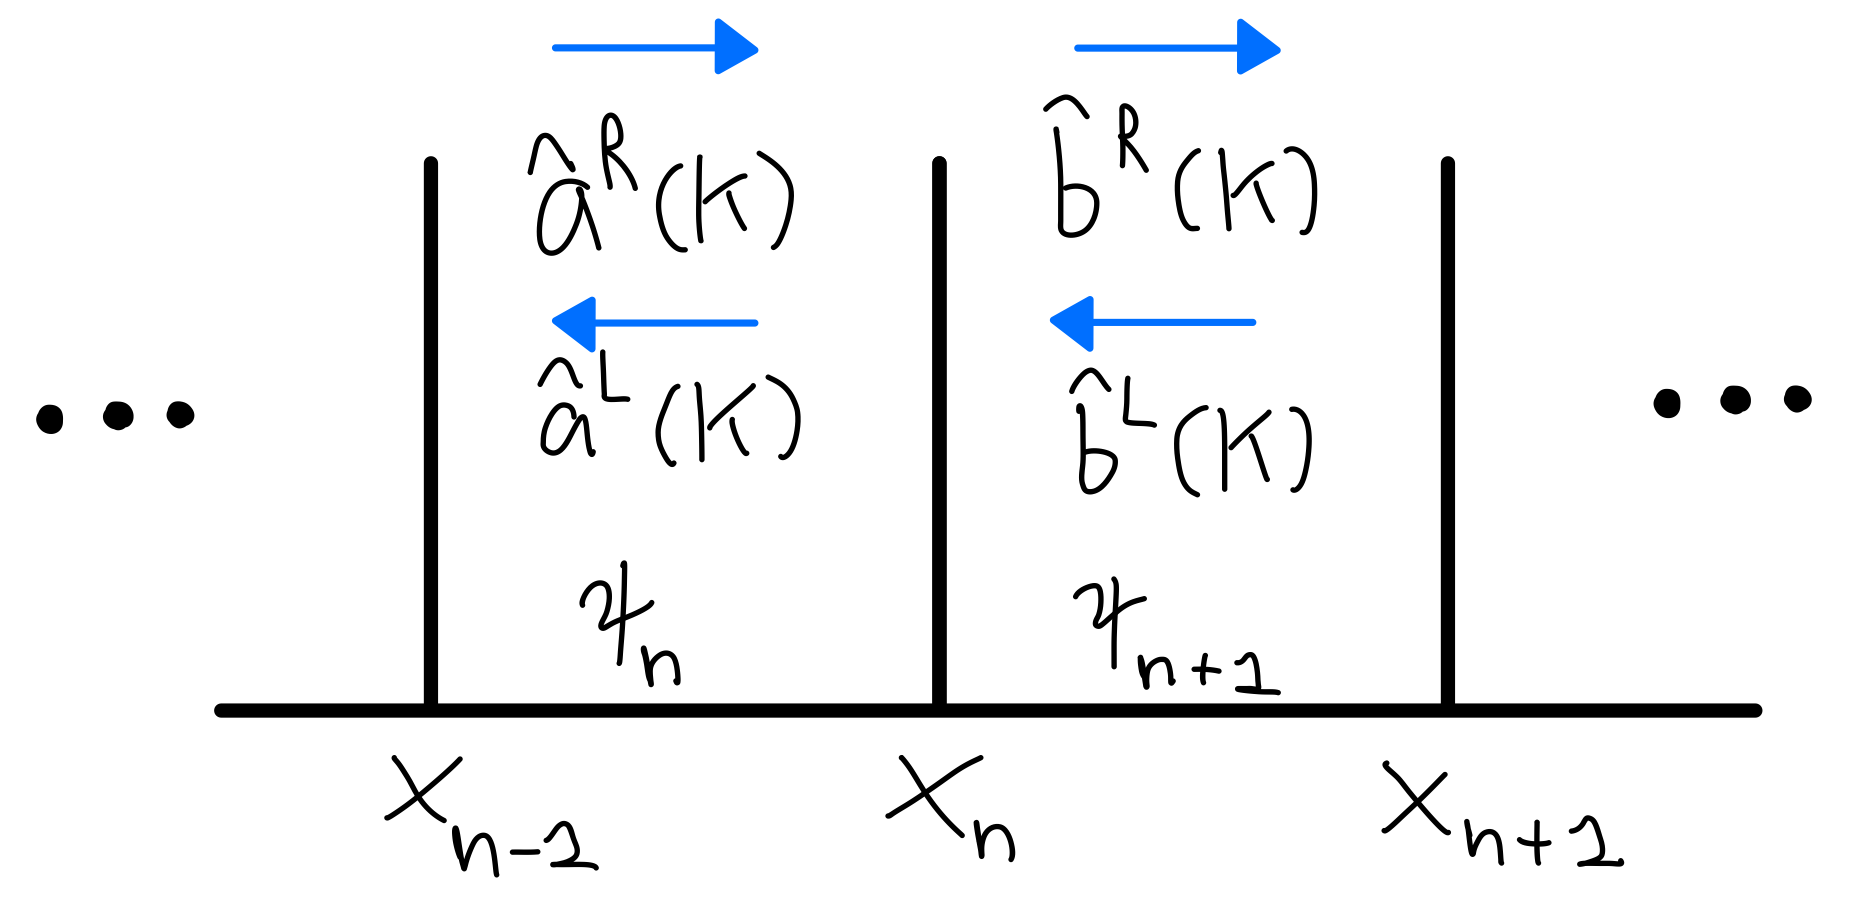
\includegraphics[width=4.5in, keepaspectratio]{figures/boundary_diagram.png}
    \caption{Diagram showing Bloch functions and creation/annihilation operators in the CPWs to the left, and right of SQUID site $n$.}
\end{figure}
%
We use the fact that the Bloch functions $\psi_K(x)$ are, by construction, eigenfunctions of the same boundary condition (see Appendix \ref{ch:appendix_bloch}). Then, we can write our boundary condition in the form
%
\begin{equation}
    \left[\hat{a}^R(K) - \hat{b}^R(K)\right]\left.\frac{\partial \psi^R_K(x)}{\partial x}\right|_{x=n^+}
    +
    \left[\hat{a}^L(K) - \hat{b}^L(K)\right]\left.\frac{\partial \psi^L_K(x)}{\partial x}\right|_{x=n^+} = 0 
\end{equation}
%
Using (eq. \ref{eq:bloch_waves}) and the relation $u_K(x) = u^*_K(x)$ (see Appendix \ref{ch:appendix_bloch}),
%
\begin{equation}\label{eq:BC_static_2}
\begin{split}
    \left[\hat{a}^R(K) - \hat{b}^R(K)\right]
    \left.
    \left\lbrace
    i K \, u_K(x) + \frac{\partial u_K(x)}{\partial x}
    \right\rbrace
    \,e^{i K x}
    \right|_{x=n}
    \\[2mm]
    +
    \left[\hat{a}^L(K) - \hat{b}^L(K)\right]
    \left.
    \left\lbrace
    -i K\, u_K(x) + \frac{\partial u_K(x)}{\partial x}
    \right\rbrace
    \,e^{-i K x} 
    \right|_{x=n}
    = 0 
\end{split}
\end{equation}
%
We now define the short hand notations
%
\begin{gather}
    \mathcal{C}_K = \left.u_K(x)\right|_{x=n}
    \label{eq:cal_C}\\
    %
    \mathcal{D}_K = \left.\frac{\partial u_K(x)}{\partial x}\right|_{x=n}
    \label{eq:cal_D}\\
    %
    \mathcal{A}_K = iK\mathcal{C}_K + \mathcal{D}_K.
    \label{eq:cal_A}
\end{gather}
%
As well as, 
\begin{subequations}\label{eq:cr_an_position_dept}
\begin{eqnarray}
    \hat{a}^R_K(x) = \hat{a}^R(K)\,e^{i K x},
    \\
    \hat{a}^L_K(x) = \hat{a}^L(K)\,e^{-i K x}. 
\end{eqnarray}
\end{subequations}
%
Similarly for $\hat{b}(K)$. We can now write a clean form for our boundary condition using (Eq. \ref{eq:cal_C} - \ref{eq:cr_an_position_dept}),
%
\begin{equation}\label{eq:BC_static_3}
    \left.\left[\hat{a}^R_K(x) - \hat{b}_K^R(x)\right]\right|_{x=n} \mathcal{A}_K
    +
    \left.\left[\hat{a}^L_K(x) - \hat{b}^L_K(x)\right]\right|_{x=n}\mathcal{A}^*_K = 0 
\end{equation}
%
We also impose the requirement that $\hat{\phi}_n(x,\mu)$ is continuous at the boundary $x=n$. Which, using (Eq. \ref{eq:bloch_waves}, we can express as,
%
\begin{equation}\label{eq:continuity_static}
    \left.\left[\hat{a}^R_K(x) + \hat{a}^L_K(x)\right]\right|_{x=n}
    =
    \left.\left[\hat{b}^R_K(x) + \hat{b}^L_K(x)\right]\right|_{x=n}
\end{equation}
%
Using (Eq. \ref{eq:BC_static_3}, \ref{eq:continuity_static}), we arrive at the relations between annihilation coefficients for static applied magnetic flux in our SQUIDs ($E_J(t)= E^0_J$),
%
\begin{subequations}\label{eq:static_solutions}
\begin{eqnarray}
    \hat{b}^R(K) = \hat{a}^R(K),
    \\
    \hat{b}^L(K) = \hat{a}^L(K).
\end{eqnarray}
\end{subequations}
%
Similar equations can be obtained for creation operators by using (Eq. \ref{eq:phi_FT_b}), for $\mu<0$. 

Note that these solutions imply that photons with allowed frequencies $\mu$, given by the band structure of the lattice (Eq. \ref{eq:bands_condition}), will pass through the whole lattice experiencing only a change in their phase. Meanwhile, photons with frequencies within the band gaps will not pass through the lattice. In this particular sense, behavior of our photons is identical to that of electrons in a solid (see Section \ref{sec:KP_in_SS}).

\section{Weak Harmonic Drive Solution}\label{eq:Static_Flux}

We now wish to analyze the dynamic version of our system, where the potential now exhibits a time dependent modulation. We use the results obtained for the static case (Eq. \ref{eq:cal_C} - \ref{eq:BC_static_3}) to write the Fourier-transformed boundary condition (Eq. \ref{eq:BC_field}) for a time-dependent Josephson energy $E_J(t)$,
%
\begin{equation}\label{eq:BC_time_dependent}
\begin{split}
    \left(\frac{\hbar}{L_0}\right)
    \frac{d\omega(K)}{\sqrt{\mu}}
    \left\lbrace
    \left.
    \left[\hat{a}^R_K(x) - \hat{b}_K^R(x)\right]
    \right|_{x=n}
    \mathcal{A}_K +
    \left.
    \left[\hat{a}^L_K(x) - \hat{b}^L_K(x)\right]
    \right|_{x=n}
    \mathcal{A}^*_K
    \right\rbrace
    \\[4mm]
    +\hspace{2mm}
    \hbar \, \left(\frac{2\pi}{\Phi_0}\right)^2
    %
    \left[
    \int_{0}^{\infty} dK'\,
    \delta g(K, K')
    \left.
    \left\lbrace \hat{a}^R_K(x) + \hat{a}_K^L(x) \right\rbrace
    \right|_{x=n}
    \mathcal{C}_K\right.
    \\[4mm]
    +
    \left.
    \int_{-\infty}^{0} dK'\,
    \delta g(K, K')
    \left.
    \left\lbrace [\hat{a}^R_K(x)]^\dagger + [\hat{a}_K^L(x)]^\dagger \right\rbrace
    \right|_{x=n}
    \mathcal{C}_K
    \right]
    = 0
    %
\end{split}
\end{equation}
%
Where we have made a change of variables to so that integration runs over $K'=K(\mu')$, separated the integral into two sections, (for positive and negative $\mu$), and defined the following
%
\begin{gather}
    d\omega (K) = 
    \left|\left.\frac{d\omega}{dK}\right|_{\omega=\mu}\right|^{-1}
    \label{eq:shorthand_dw}
    \\
    \delta g(\mu, \mu') = \frac{1}{2 \pi} \sqrt{\frac{|\mu|}{|\mu'|}}
    \int_{-\infty}^{\infty} dt \, \epsilon(t) \, e^{i(\mu - \mu')t}
    \label{eq:energy_FT}
    \\
    g(\mu, \mu') =  \frac{1}{2 \pi} \sqrt{\frac{|\mu|}{|\mu'|}}
    \int_{-\infty}^{\infty} dt \, E_J(t) \, e^{i(\mu - \mu')t}
    = E_J^0 + \delta g(\mu, \mu').
\end{gather}
%
We proceed to drive our system by applying an external flux equally to all of the SQUID sites, such that the form of the time-dependent Josephson energy (Eq. \ref{eq:energyexp1}), where the drive is in phase $\varphi_n=0$ is:
%
\begin{equation}\label{eq:time_dependent_energy}
\begin{split}
    E_J(t) = E^0_J + \epsilon(t),
    \\
    \text{where,} \hspace{2mm}
    \epsilon(t) = \delta E^0_J \cos(\Omega t). 
\end{split}
\end{equation}
%
We consider a weak harmonic drive, such that $\frac{\delta E^0_J}{E^0_j} \ll 1$. Then, the
%
\begin{equation}
    \delta g(\mu, \mu') =
    \frac{\delta E_J^0}{2}
    \sqrt{\frac{|\mu|}{|\mu'|}}
    \left[
    \delta (\mu' - \mu - \Omega) +
    \delta(\mu' - \mu + \Omega)
    \right]
\end{equation}
%
or, in terms of $K$,
\begin{equation} \label{eq:dw_K_continuous}
    \delta g(K,K')= 
    \frac{\delta E_J^0}{2}
    \sqrt{\frac{|\mu|}{|\mu'|}}
    d\omega (K')
    \left[
    \delta (K' - K_+) + \delta(K' - K_-)
    \right]
\end{equation}
% 
where we have used the shorthand notations,
%
\begin{gather}
    K_+ = K(\mu + \Omega),\\
    %
    K_- = K(\mu - \Omega).
\end{gather}
%

\section{Numerical Calculation, Band Structure, and Reduced Domains}

In order to obtain a transfer matrix for our system, we need a relation between operators right and left of our boundary. To do this we use our boundary condition (Eq. \ref{eq:BC_time_dependent}), truncate the frequency range to $[-\Omega, \Omega]$ and discretizing it in $(2 N_{\Omega} + 1)$ steps $[-\omega_N, ..., \omega = 0, ..., \omega_N]$ where $\omega_N = \Omega$. 

We parametrize as $\omega_n = \omega + (N_{\Omega} + 1 - n)$, where $n = 1, ..., 2N_{\Omega}+1$, and define $K_n = K(|\omega_n|)$, $d \omega (n) = d \omega(K_n)$, similarly for $\mathcal{A}_n = \mathcal{A}_{K_n}, \mathcal{C}_n = \mathcal{C}_{K_n}$. We can now write, 
%
\begin{equation}\label{eq:BC_discrete_1}
\begin{split}
    \left(\frac{1}{L_0}\right)
    d\omega(n)
    \left\lbrace
    \left[\hat{a}_R(n) - \hat{b}_R(n)\right]
    \mathcal{A}_n 
    +
    \left[\hat{a}_L(n) - \hat{b}_L(n)\right]
    \mathcal{A}^*_n
    \right\rbrace
    \\[4mm]
    +\hspace{2mm}
    \left(\frac{2\pi}{\Phi_0}\right)^2
    %
    \left[
    \sum_{m=-N}^{N} \Delta K_m\,
    \delta g_{m, n}
    d \omega(m)
    \left\lbrace \hat{a}_R(m) + \hat{a}_L(m) \right\rbrace
    \mathcal{C}_m\right.
    \\[4mm]
    +
    \left.
    \sum_{m=-N}^{N} \Delta K_m\,
    \delta g_{m, n}
    d \omega(m)
    \left\lbrace [\hat{a}_R(m)]^\dagger + [\hat{a}_L(m)]^\dagger \right\rbrace
    \mathcal{C}_m
    \right]
    = 0
    %
 \end{split}
\end{equation}
%
\begin{equation}
    \delta g(n,m)= 
    \frac{\delta E_J^0}{2}
    \sqrt{\frac{|\omega_n|}{|\omega_m|}}
    \left[ 
    d\omega (n+1) \delta_{m, n+1}
    + d\omega (n-1) \delta_{m, n-1}
    \right]
\end{equation}
%
Multiplying both sides by $\left(\frac{\Phi_0}{2\pi}\right)^2 \frac{1}{E_J^0}$ and using 
\begin{equation}
    L_{\text{eff}} = \left(\frac{\Phi_0}{2\pi}\right)^2 \frac{1}{E_J^0 L_0}
\end{equation}
%
\begin{equation}\label{eq:BC_discrete_2}
\begin{split}
    L_{\text{eff}}\, 
    d\omega(n)
    \left\lbrace
    \left[\hat{a}_R(n) - \hat{b}_R(n)\right]
    \mathcal{A}_n 
    +
    \left[\hat{a}_L(n) - \hat{b}_L(n)\right]
    \mathcal{A}^*_n
    \right\rbrace
    \\[4mm]
    +\hspace{2mm}
    \frac{\delta E_J^0}{2 E_J^0}
    %
    \sum_{m=1}^{2N_{\Omega}+1}
    \sqrt{\frac{|\omega_n|}{|\omega_m|}}
    d \omega(m)
    \left[ 
    \delta_{m, n+1}
    + \delta_{m, n-1}
    \right]
    \\[4mm]
    *
    \left[
    \Theta(\omega_n)
    \left\lbrace \hat{a}_R(m) + \hat{a}_L(m) \right\rbrace
    \mathcal{C}_m
    +
    \Theta(-\omega_n)
    \left\lbrace [\hat{a}_R(m)]^\dagger + [\hat{a}_L(m)]^\dagger \right\rbrace
    \mathcal{C}_m
    \right]
    = 0
    %
 \end{split}
\end{equation}